\section{Scire, Potere, Audere, Tacere}

\begin{quotex}
\emph{Scire, Potere, Audere, Tacere}

To know, to be able, to dare, to keep silent

\flright{\textsc{Zoroaster}} 

\end{quotex}

\begin{wrapfigure}{rt}{0.35\textwidth}
\centering
 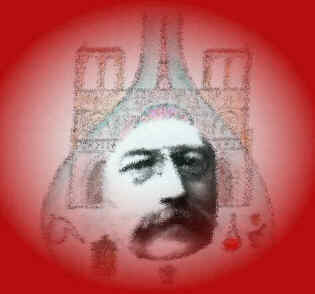
\includegraphics[scale=.25]{a20100928ScirePotereAudereTacere-img001.jpg} 
\end{wrapfigure}

Nature does not open the door of the sanctuary to anyone.

In these pages, the uninitiated will perhaps discover some proof of a genuine and positive science. I do not however, flatter myself that I shall convert them, for I know full well the obstinacy of prejudice and the great strength of preconceived opinions. The disciple will derive greater benefit form this book, provided always that he does not despise the works of the old Philosophers and that he studies with care and penetration the classical text, until he has acquired sufficient perception to understand the obscure points of the practice.

No one may aspire to possess the great secret, if he does not direct his life in accordance with the researches he has undertaken.

It is not enough to be studious, active, and persevering, if one has no firm principles, no solid basis, if immoderate enthusiasm blinds one to reason, if pride overrules judgment, if greed expands before the prospect of a golden future.

The mysterious science requires great precision, accuracy and perspicacity in observing the facts, a healthy, logical and reflective mind, a lively but not over-excitable imagination, a warm and pure heart. It also demands the greatest simplicity and complete indifference with regard to theories, systems and hypotheses, which are generally accepted without question on the testimony of books or the reputation of their authors, it requires its candidates to learn to think more with their own brains and less with those of others. Finally, it insists that they should check the truth of its principles, the knowledge of its doctrine and the practice of its operations from nature, the mother of us all.

By constant exercise of the faculties of observation and reasoning and by meditation, the novice will climb the steps leading to 

\paragraph{Knowledge}
A simple imitation of natural processes, skill combined with ingenuity, the insight born of long experience will secure for him

\paragraph{Power}
Having obtained that, he will still have need of patience, constancy and unshakeable will. Brave and resolute, he will be enabled by the certainty and confidence born of a strong faith, to

\paragraph{Dare}
Finally, when success has crowned so many years of labour, when his desires have been accomplished, the Wise Man, despising the vanities of the world, will draw near to the humble, the disinherited, to all those who work, suffer, struggle and weep here below. As an anonymous and dumb disciple of eternal Nature, he will remain faithful to his vow of silence. In Science, in Goodness, the adept must evermore

\paragraph{Keep Silent}

\flrightit{Posted on 2010-09-28 by Cologero }

\begin{center}* * *\end{center}

\begin{footnotesize}\begin{sffamily}



\texttt{Niko The Exile on 2019-02-15 at 00:18 said: }

This is exceptional, this so much reminds one of the Desert Fathers, i wonder if they were on the same wavelength as Fulcanelli.


\end{sffamily}\end{footnotesize}
